\documentclass{beamer}
\usepackage[utf8]{inputenc}
\usepackage{hyperref}
\usepackage[czech]{babel}
\usetheme{AnnArbor}
\usecolortheme{crane}
\usepackage[czech]{algorithm2e}


\title{Insertion Sort}
\author[Zlevorová]{Martina Zlevorová (xzlevo00)}
\institute[VUT FIT]{Fakulta informačních technologií\\
Vysoké učení technické v Brně}
\date{\today}
\subject{Computer Science}

\begin{document}
\frame{\titlepage}
\begin{frame}{Řazení\,--\,Definice}
\uv{\emph{Řazení je proces vytvoření určitého pořadí (seřazení) různých objektů podle nějaké veličiny (číselná hodnota, pořadí v abecedě). Řazení je typicky závislé na národních zvyklostech (pořadí písmen v abecedě, ohled na velká či malá písmena), na úhlu pohledu, na zvyklosti v daném oboru (knihovnictví).}}\cite{wiki}
\end{frame}
\begin{frame}{Řadicí algoritmy}
\begin{itemize}
\item Selection Sort
\item Insertion Sort
\item Bubble Sort
\item Quick Sort
\item Merge Sort
\item \dots
\end{itemize}
\end{frame}
\begin{frame}{Insertion Sort (Řazení vkládáním)}
\begin{itemize}
\pause
\item pole tvoří dvě části\,--\,setřízená a nesetřízená
\pause
\item na začátku je v setřízené části jen první prvek
\pause
\item postupně porovnáváme první prvek nesetřízené části s prvky v~setřízené části, dokud nedojdeme na místo, kam by se měl zařadit
\pause
\begin{itemize}
\item při porovnávání posunujeme čísla větší než zařazovaný prvek o~1~doprava
\pause
\item dokud nenarazíme na prvek menší nebo roven zařazovanému prvku
\end{itemize}
\end{itemize}
\end{frame}

\begin{frame}{Insertion Sort\,--\,Ukázka}
\begin{figure}[H]
\centering
\scalebox{0.33}{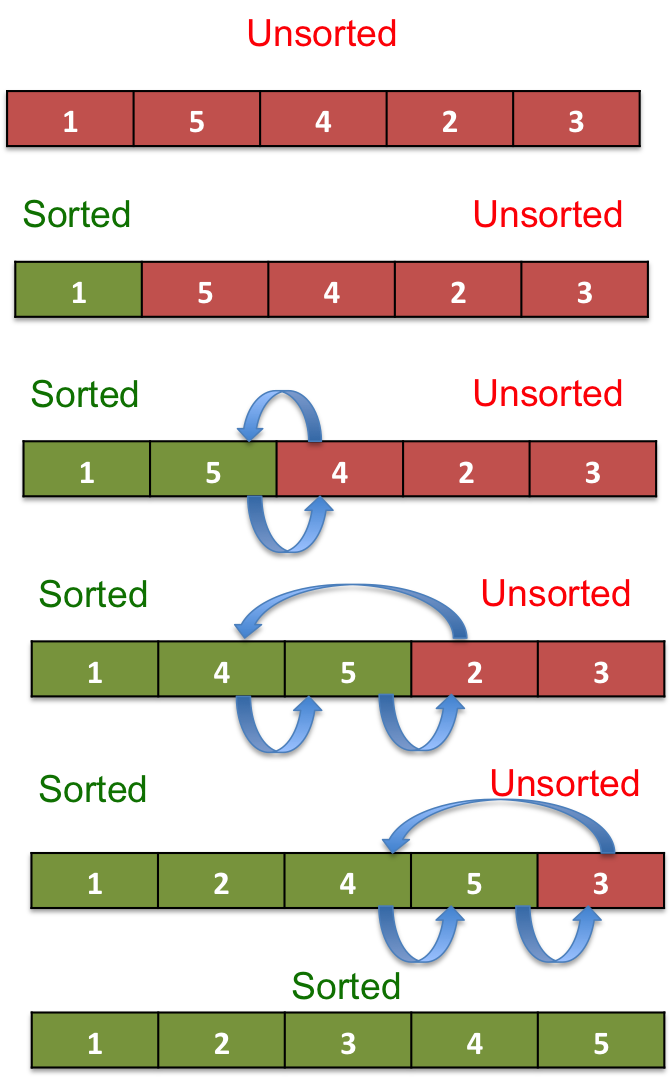
\includegraphics{ISort.png}}
\caption{Insertion Sort \cite{hacr}}
\label{fig:IS}
\end{figure}
\end{frame}

\begin{frame}{Insertion Sort\,--\,Pseudokód}
\begin{algorithm}[H]
\TitleOfAlgo{Insertion Sort}
\SetAlgoLined
\DontPrintSemicolon
\SetKwFor{For}{for}{do}{end\ for}
\For{$j \gets 1 \textbf{ to } n - 1$}{
    $t \gets$ $A$[\,$j$\,]\;
    $i \gets$ $j - $1\;
    \While{$i \geq 0 \land A[\,i\,] > t$}{
        $A[\,i+1\,] \gets A[\,i\,]$\;
        $i \gets i-1$\;
    }
    $A[\,i+1\,] \gets t$
}

\end{algorithm}
\end{frame}

\begin{frame}{Zdroje}
\begin{thebibliography}{9}
\bibitem{wiki}
Přispěvatelé Wikipedie. Řazení [online]. Wikipedie: Otevřená encyklopedie, c2018, [rev. 9. 04. 2018], [vid. 29. 04. 2019] Dostupné z: \href{https://cs.wikipedia.org/wiki/Řazení}{https://cs.wikipedia.org/wiki/Řazení}

\bibitem{hacr}
HackerRank. Insertion Sort. Dostupné z: \href{https://www.hackerrank.com/topics/insertion-sort}{https://www.hackerrank.com/topics/insertion-sort}

\end{thebibliography}
\end{frame}
\end{document}
